\section{Performance Results with Graphs}

In this section, we compare a serial C++ baseline, unbatched and batched PyTorch baselines, and our custom parallel CUDA implementation to analyze forward-pass runtime across configurations. We evaluate these methods under three scaling regimes: (i) fixed model size with increasing number of names processed, (ii) fixed number of names with increasing model size, and (iii) scaling both simultaneously.

We do not directly compare performance between our CUDA implementation and \textit{microgpt}, as the pure Python implementation is prohibitively slow (our CUDA implementation is over 10{,}000$\times$ faster on a medium benchmark). However, we use \textit{microgpt} to validate correctness by comparing logits from a single-sequence forward pass against those produced by the original implementation. 

For analyzing results, we will abbreviate methods as UT = unbatched\_torch, BT = batched\_torch, SC = serial\_cpp, and PC = parallel\_cpp. We abbreviate presets as S, M, L, VL, and XL for the standard size sweep, and MS5, MM5, ML5, MVL5, and MXL5 for the 5k-step model sweep.

We begin by examining the case of a fixed model size with increasing input name counts, shown in Figure \ref{result:1} below. 

Our PC method outperforms all other baselines across every input size benchmarked. For both SC and UT, this result is unsurprising, as PC is more heavily optimized for this specific workload. More notably, PC also outperforms BT, which is a highly optimized and widely used ML framework. This advantage can largely be attributed to Python overhead in BT, including costs associated with object management and data movement between Python and underlying implementations.

However, a closer examination of the results shows that, while PC currently outperforms BT, its runtime increases more rapidly with input size, whereas BT exhibits near-ideal scaling behavior. It is therefore reasonable to expect that as input sizes continue to grow, particularly to those typical of modern ML workloads, PC will eventually lose its performance advantage.

\begin{figure}[h]
    \centering
    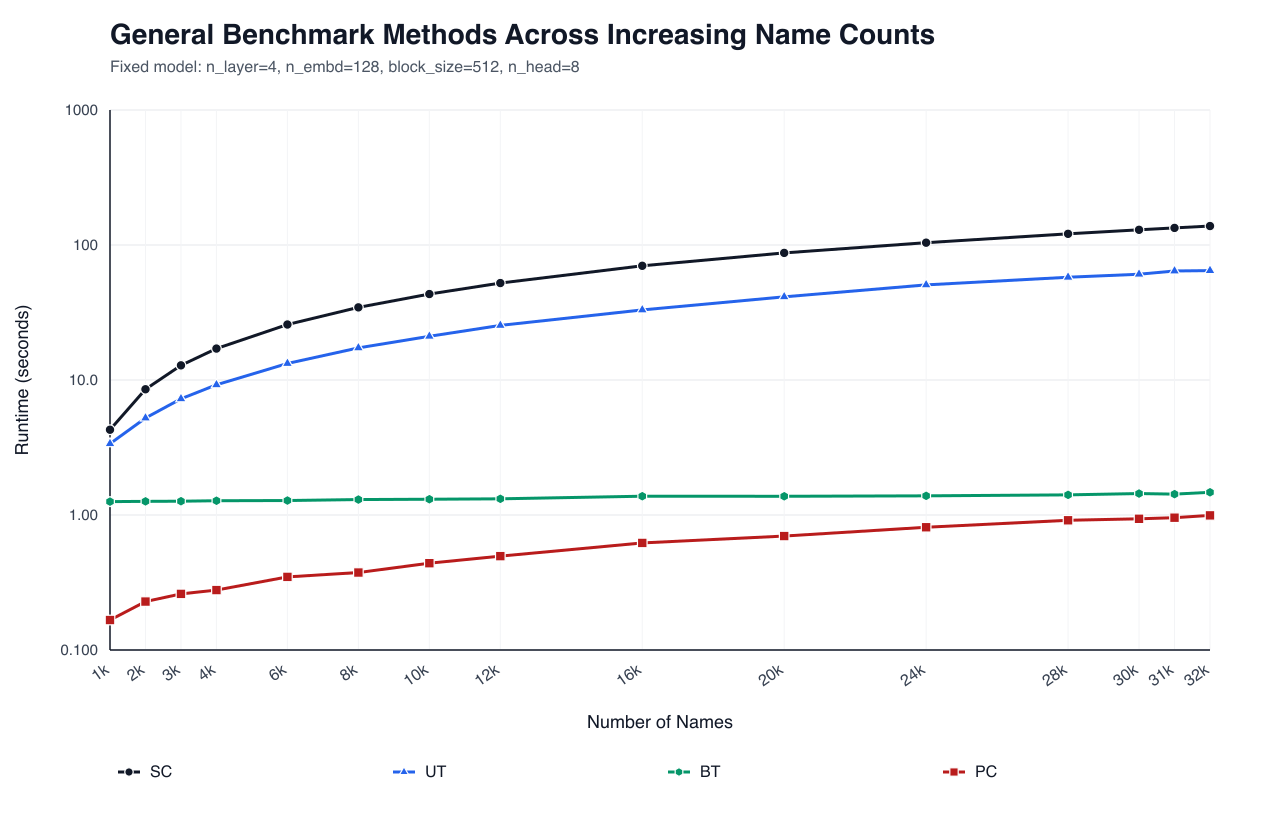
\includegraphics[width=0.6\linewidth]{figures/general_benchmark_names.png}
    \caption{Results from Input Scaling}
    \label{result:1}
\end{figure}


Next we will look the results from both our other scaling approaches: holding input size constant while increasing the model size ref, and increasing both the input size and model size ref. The model presets both of these expierments are presents below in table \ref{tab:model_configs} 


\begin{table}[H]
\centering
\begin{tabular}{lccccc}
\hline
\textbf{Preset} & \textbf{n\_layer} & \textbf{n\_embd} & \textbf{block\_size} & \textbf{n\_head} & \textbf{steps} \\
\hline

\hline
S            & 1 & 64  & 128 & 4  & 200   \\
M            & 2 & 128 & 128 & 8  & 1000  \\
L            & 4 & 256 & 256 & 8  & 2500  \\
VL           & 6 & 384 & 512 & 12 & 5000  \\
XL           & 8 & 512 & 512 & 16 & 10000 \\

\hline
MS5          & 1 & 64  & 512 & 4  & 5000 \\
MM5          & 2 & 128 & 512 & 8  & 5000 \\
ML5          & 4 & 256 & 512 & 8  & 5000 \\
MVL5         & 6 & 384 & 512 & 12 & 5000 \\
MXL5         & 8 & 512 & 512 & 16 & 5000 \\

\hline
\end{tabular}
\caption{Model Configurations Used in Experiments}
\label{tab:model_configs}
\end{table}


\begin{table}[h]
\centering

\begin{minipage}{0.49\textwidth}
\centering
\begin{tabular}{l c c c c}
\toprule
\textbf{Preset} & \textbf{UT} & \textbf{BT} & \textbf{SC} & \textbf{PC} \\
\midrule

S  & \makecell{1.04 \\ $0.06\times$}
   & \makecell{0.89 \\ $0.07\times$}
   & \makecell{0.06 \\ $1.00\times$}
   & \makecell{0.11 \\ $0.58\times$} \\

M  & \makecell{2.17 \\ $0.99\times$}
   & \makecell{1.05 \\ $2.06\times$}
   & \makecell{2.16 \\ $1.00\times$}
   & \makecell{0.15 \\ $14.46\times$} \\

L  & \makecell{7.36 \\ $6.33\times$}
   & \makecell{2.33 \\ $19.98\times$}
   & \makecell{46.56 \\ $1.00\times$}
   & \makecell{0.37 \\ $125.21\times$} \\

VL & \makecell{20.10 \\ $16.29\times$}
   & \makecell{5.78 \\ $56.69\times$}
   & \makecell{327.49 \\ $1.00\times$}
   & \makecell{1.04 \\ $315.81\times$} \\

XL & \makecell{51.34 \\ $30.77\times$}
   & \makecell{12.51 \\ $126.27\times$}
   & \makecell{1579.67 \\ $1.00\times$}
   & \makecell{3.51 \\ $450.23\times$} \\

\bottomrule
\end{tabular}
\end{minipage}
\hspace{0.001\textwidth}  % adjust this
\begin{minipage}{0.48\textwidth}
\centering
\begin{tabular}{l c c c c}
\toprule
\textbf{Preset} & \textbf{UT} & \textbf{BT} & \textbf{SC} & \textbf{PC} \\
\midrule

MS5 & \makecell{4.33 \\ $0.28\times$}
    & \makecell{0.92 \\ $1.34\times$}
    & \makecell{1.23 \\ $1.00\times$}
    & \makecell{0.20 \\ $6.22\times$} \\

MM5 & \makecell{6.81 \\ $1.58\times$}
    & \makecell{1.10 \\ $9.80\times$}
    & \makecell{10.76 \\ $1.00\times$}
    & \makecell{0.26 \\ $41.38\times$} \\

ML5 & \makecell{12.45 \\ $7.51\times$}
    & \makecell{2.37 \\ $39.45\times$}
    & \makecell{93.53 \\ $1.00\times$}
    & \makecell{0.50 \\ $185.50\times$} \\

MVL5 & \makecell{20.20 \\ $16.21\times$}
     & \makecell{5.79 \\ $56.50\times$}
     & \makecell{327.28 \\ $1.00\times$}
     & \makecell{1.07 \\ $307.03\times$} \\

MXL5 & \makecell{32.29 \\ $24.30\times$}
     & \makecell{12.34 \\ $63.59\times$}
     & \makecell{784.64 \\ $1.00\times$}
     & \makecell{2.10 \\ $373.60\times$} \\

\bottomrule
\end{tabular}
\end{minipage}

\caption{Runtime (top) and speedup (bottom) per method. \textbf{Speedup is relative to SC}}
\end{table}